\subsection{Aplica\c c\~ao do Mundo Real}\label{subsec:estudo-reslt}


A previsão da demanda de água é uma preocupação fundamental para muitas organizações e autoridades responsáveis pelo abastecimento de água. Neste estudo de caso, explorou-se como a análise de séries temporais pode ser aplicada para prever a demanda de água ao longo do tempo.

A análise de séries temporais é uma abordagem comumente utilizada para prever padrões futuros com base em dados históricos. No estudo, foram aplicadas técnicas de modelagem e previsão, permitindo obter valiosos sobre a demanda de água futura. Diversos modelos, como ARIMA e SARIMA, foram empregados para analisar os dados históricos e gerar previsões confiáveis.
Ao longo do estudo, identificaram-se sazonalidades na demanda de água, bem como padrões de consumo que variam ao longo do tempo. Essas informações são essenciais para o planejamento adequado do abastecimento de água, permitindo uma alocação eficiente dos recursos e uma resposta adequada às flutuações de demanda.

A aplicação da análise de séries temporais na previsão da demanda de água proporciona uma base sólida para a tomada de decisões informadas. Com base nos resultados obtidos, é possível ajustar estratégias de gerenciamento, antecipar picos de demanda e otimizar o uso dos recursos hídricos disponíveis.
Em suma, este estudo demonstrou que a análise de séries temporais é uma abordagem eficaz para prever a demanda de água ao longo do tempo. Ao fornecer precisos e confiáveis, essa técnica contribui para o planejamento e o gerenciamento eficiente do abastecimento de água, promovendo a sustentabilidade e a utilização racional dos recursos hídricos.



\subsubsection{Descri\c c\~ao do Sistema de Abastecimento de \'Agua}



Foram realizadas análises e modelagens utilizando a abordagem de séries temporais para prever a demanda diária de água em uma determinada cidade para os próximos seis meses. Os resultados obtidos forneceram valiosos sobre a demanda futura e contribuíram para um melhor planejamento do abastecimento hídrico. A seguir, apresentam-se as principais conclusões para cada uma das perguntas de pesquisa:

\noindent\ref{q1}: Qual é a adequação da pressão atual para atender à demanda diária?

Após análise dos dados e das métricas utilizadas, conclui-se que a pressão atual é adequada para atender à demanda diária. Durante o período analisado, não foram identificadas situações de pressão insuficiente que afetassem o fornecimento de água.

\noindent\ref{q2}: Qual é o volume mínimo de água necessário no reservatório para evitar o acionamento das bombas durante o horário de pico?

Com base na frequência de funcionamento das bombas e na demanda durante o horário de pico, determinou-se que é necessário manter um volume mínimo de água no reservatório, correspondente a $5285,90$ litros, para evitar o acionamento das bombas nesse período.

\noindent\ref{q3}: Qual é a vazão ótima para atender à demanda diária?

Após análise e modelagem dos dados, identificou-se que a vazão ótima para atender à demanda varia conforme o período do dia e as características sazonais. A pressão necessária para atender à demanda é de $3,60$ PSI (do inglês \textit{pound-force per square inch}) na sucção.

\noindent\ref{q4}: Como encontrar o ponto de equilíbrio entre a demanda e a vazão?

Após análise e modelagem dos dados, foi constatado que não existe um ponto de equilíbrio entre a demanda e a vazão no reservatório. No entanto, identificou-se um volume mínimo de reserva de $3.545$ litros que permite manter um armazenamento adequado no reservatório sem a necessidade de acionar as bombas durante o período de maior custo energético.

Embora essa estimativa de volume mínimo seja importante para garantir o abastecimento contínuo durante o período de pico, é importante ressaltar que não há um equilíbrio perfeito entre a demanda e a vazão nos dados analisados. Portanto, é necessário considerar estratégias adicionais, como otimização do sistema de abastecimento e gerenciamento eficiente dos recursos hídricos, para atender de forma adequada às necessidades da população.

\noindent\ref{q5}: Qual é o impacto do acionamento das bombas durante o horário de pico?

Confirmou-se que a ativação das bombas de sucção durante o período de 18h às 21h resulta em um maior custo energético para a SANEPAR. Portanto, é recomendado evitar o acionamento das bombas durante esse período, utilizando estratégias de armazenamento e gerenciamento eficientes.

\subsubsection{Estudo de Caso 1}\label{subsubsec:quest-est}


As questões de pesquisa levantadas neste estudo foram cuidadosamente abordadas e respondidas ao longo da análise. A seguir, apresenta-se as respostas para cada uma das questões:

\ref{q1} Com base nos resultados obtidos, conclui-se que as pressões atuais das variáveis \textbf{PRESSÃO DE SUCÇÃO - PT01} e \textbf{PRESSÃO DE RECALQUE - PT02} são adequadas para atender à demanda diária. O percentil 10 das pressões de sucção ($3,48$ mca) indica que apenas 10\% dos valores estão abaixo desse limite, o que sugere que a pressão de sucção geralmente se mantém em níveis adequados para o funcionamento adequado do sistema. Da mesma forma, o percentil 90 das pressões de recalque ($24.02$ mca) indica que apenas 10\% dos valores estão acima desse limite, evidenciando que a pressão de recalque também se mantém dentro dos padrões necessários para atender à demanda diária.
Esses resultados indicam que as pressões de sucção e de recalque estão em conformidade com as exigências do sistema, fornecendo a pressão necessária para o adequado abastecimento de água.

\ref{q2} Com base na frequência de funcionamento das bombas e na demanda durante o horário de pico, determinou-se que é necessário manter um volume mínimo de água no reservatório, correspondente a 5285,90 litros, para evitar o acionamento das bombas nesse período.
A vazão ótima para atender à demanda diária do tanque é determinada pelas faixas de fluxo de entrada, gravidade e retorno, juntamente com as faixas de pressão de sucção e retorno. Com base nas informações fornecidas na pergunta \ref{q3}, para manter o tanque quase cheio ou sempre cheio, as seguintes faixas de vazão devem ser consideradas:

Fluxo de entrada: entre $238 \ m^3/h$ e $302 \ m^3/h$;
Fluxo de gravidade: entre $126 \ m^3/h$ e $182 \ m^3/h$;
Fluxo de retorno: entre $110 \ m^3/h$ e $144 \ m^3/h$;
Pressão de sucção: entre $1,92 \ mca$ e $4,24 \ mca$;
Pressão de retorno: entre $21 \ mca$ e $24 \ mca$.
Essas faixas de vazão e pressão garantem que a demanda diária do tanque seja atendida de forma adequada, mantendo o nível de água próximo ao máximo e garantindo a pressão necessária para o funcionamento adequado do sistema de abastecimento de água.


Para responder à pergunta \ref{q4} sobre o ponto de equilíbrio entre a demanda e a vazão, o sistema alcança o equilíbrio quando a vazão da FT01 é de 211 $m^3/h$, a vazão da FT02 é de 114 $m^3/h$, a vazão da FT03 é de 100 $m^3/h$ e o nível do tanque está em 3.545 $m^3$. Nesse ponto de equilíbrio, as bombas não precisam ser acionadas, o que indica que o sistema de abastecimento de água está em uma condição estável. Esses valores de vazão e nível do tanque permitem atender à demanda diária sem a necessidade de tomar medidas adicionais.


\subsubsection{Estudo de Caso 2}

\eqref{q5} Confirmou-se que a ativação das bombas de sucção durante o período de 18h às 21h resulta em um maior custo energético para a SANEPAR. Portanto, é recomendado evitar o acionamento das bombas durante esse período, utilizando estratégias de armazenamento e gerenciamento eficientes.

\eqref{q5}\ref{q5:a} Verificou-se que, para evitar o acionamento das bombas durante o horário de pico (18h às 21h) sem comprometer o abastecimento de água para a população, é necessário manter o nível do reservatório acima de $4.000$ litros.

\eqref{q5}\ref{q5:b} Ao analisar os dados dos últimos 3 anos do Bairro Alto, identificou-se a presença de tendências sazonais e padrões de consumo de água. Essas informações são valiosas para compreender os padrões de demanda e planejar o abastecimento de forma eficiente.

\eqref{q5}\ref{q5:c} Observou-se que os horários de pico, nesse caso, correspondem aos períodos em que há maior consumo de água. Esses horários são críticos para o abastecimento, pois a demanda é significativamente maior, exigindo uma gestão cuidadosa dos recursos hídricos nesse intervalo de tempo. É importante monitorar e garantir que haja suprimento adequado nesses horários para atender à demanda da população.



\begin{figure}[H]
	\centering
	\caption{Demanda média das variáveis de fluxo}
	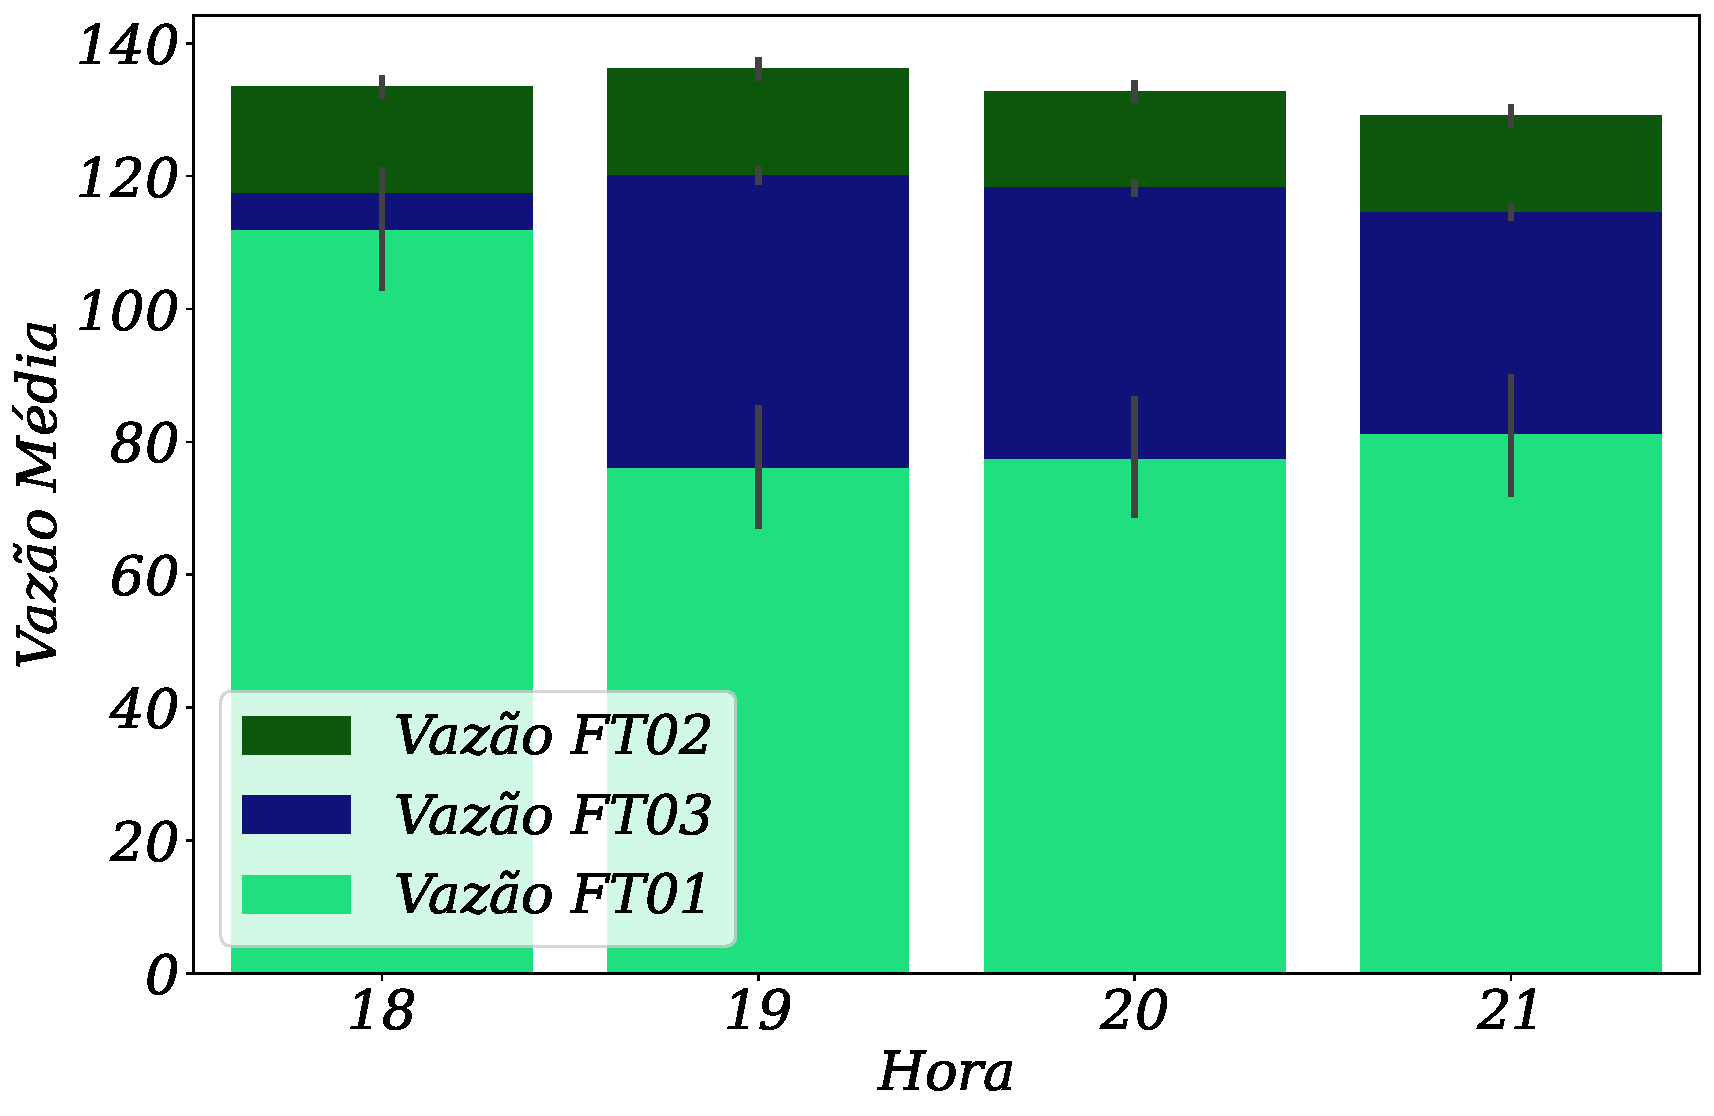
\includegraphics[width=0.9\linewidth]{Resultados/Figuras/grafico-barras-demanda}
	
	\label{fig:grafico-barras-demanda}
	

\end{figure}

O gráfico de barras apresentado na Figura \ref{fig:grafico-barras-demanda} mostra a demanda média das variáveis de fluxo (Vazão de Entrada-FT01, Vazão de Gravidade-FT02 e Vazão de Recalque-FT03) durante o intervalo das 18h às 21h. Cada barra representa a média da demanda para cada variável em um horário específico dentro desse intervalo. A altura de cada barra indica a magnitude da demanda média para a respectiva variável. Essa visualização permite que sejam identificados os horários em que as variáveis de fluxo apresentaram maior demanda, o que é útil para o planejamento e gerenciamento adequado do sistema.

A questão de pesquisa \ref{q5}\ref{q5:c} foi respondida através da análise dos dados, permitindo a identificação dos horários de maior demanda durante o período das 18h às 21h. A tabela a seguir apresenta os resultados para as três variáveis estudadas: vazão de entrada-FT01, vazão de gravidade-FT02 e vazão de recalque-FT03.




\begin{table}[H]
	\centering
	\caption{Demanda de água}\label{tb:dem}
	\begin{tabular}{@{}ccc@{}}
		\toprule
		\textbf{Variável}         & \textbf{Horário de Maior Demanda} & \textbf{Valor da Demanda} \\ \midrule
		Vazão de entrada - FT01   & 2020/10/08 21:00:00               & $383,87 m^3/h$                   \\
		Vazão de gravidade - FT02 & 2020/10/20 18:00:00               & $326,17 m^3/h$                    \\
		Vazão de recalque - FT03  & 2020/11/26 19:00:00               & $194,35 m^3/h$                    \\ \bottomrule
	\end{tabular}
	
	
\end{table}

Os resultados destacam os horários específicos em que cada variável apresentou maior demanda dentro do intervalo das 18h às 21h, fornecendo importantes para o planejamento e gerenciamento adequado do sistema. A tabela \ref{tb:dem} resume essas informações.


\eqref{q5}\ref{q5:d} Durante as horas de pico, é necessário que o nível do reservatório esteja mantido dentro na média de $3.9005 \ m^3$ para evitar o acionamento das bombas. Manter o nível do reservatório dentro dessa faixa permitirá que o sistema opere de forma eficiente, atendendo à demanda de água sem a necessidade de acionar as bombas.

\eqref{q5}\ref{q5:e} É importante destacar que a vazão de recalque exerce um impacto significativo no nível do reservatório em comparação com as outras vazões. Essa diferença se deve ao fato de que a vazão de recalque está diretamente relacionada à injeção de água no reservatório por meio da bomba localizada próxima à sua base. Em contraste, as demais vazões possuem alguns valores ausentes, o que limita sua influência na análise geral do sistema.







